\documentclass[11pt]{article}
\usepackage{setspace}
\setstretch{1}
\usepackage{amsmath,amssymb, amsthm}
\usepackage{graphicx}
\usepackage{bm}
\usepackage[hang, flushmargin]{footmisc}
\usepackage[colorlinks=true]{hyperref}
\usepackage[nameinlink]{cleveref}
\usepackage{footnotebackref}
\usepackage{url}
\usepackage{listings}
\usepackage[most]{tcolorbox}
\usepackage{inconsolata}
\usepackage[papersize={8.5in,11in}, margin=1in]{geometry}
\usepackage{float}
\usepackage{caption}
\usepackage{esint}
\usepackage{url}
\usepackage{enumitem}
\usepackage{subfig}
\usepackage{wasysym}
\newcommand{\ilc}{\texttt}
\newcommand{\p}{\partial}
\usepackage{etoolbox}
\usepackage{algorithm}
\usepackage{changepage}
% \usepackage{algorithmic}
\usepackage[noend]{algpseudocode}
\usepackage{tikz}


\usetikzlibrary{matrix,positioning,arrows.meta,arrows}
\patchcmd{\thebibliography}{\section*{\refname}}{}{}{}
% \PassOptionsToPackage{hyphens}{url}\usepackage{hyperref}

\providecommand{\myceil}[1]{\left \lceil #1 \right \rceil }
\providecommand{\myfloor}[1]{\left \lfloor #1 \right \rfloor }
\providecommand{\qbm}[1]{\begin{bmatrix} #1 \end{bmatrix}}
\providecommand{\qpm}[1]{\begin{pmatrix} #1 \end{pmatrix}}
\providecommand{\norm}[1]{\left\lVert #1 \right\rVert}
\providecommand{\len}[1]{\left| #1 \right|}
\newcommand{\cmark}{\ding{51}}%
\newcommand{\xmark}{\ding{55}}%

\definecolor{dkgreen}{rgb}{0,0.6,0}
\definecolor{gray}{rgb}{0.5,0.5,0.5}
\definecolor{mauve}{rgb}{0.58,0,0.82}

\lstset{frame=tb,
  language=Python,
  aboveskip=3mm,
  belowskip=3mm,
  showstringspaces=false,
  columns=flexible,
  basicstyle={\small\ttfamily},
  numbers=none,
  numberstyle=\tiny\color{gray},
  keywordstyle=\color{blue},
  commentstyle=\color{dkgreen},
  stringstyle=\color{mauve},
  breaklines=true,
  breakatwhitespace=true,
  tabsize=3
}

\begin{document}


\title{\textbf{CSDS 491: Assignment 4}}

\author{Shaochen (Henry) ZHONG, \ilc{sxz517@case.edu}}

\date{Due and submitted on 04/21/2021 \\ Spring 2021, Dr. Lewicki}
\maketitle

\section*{E1. Multivariate Gaussians}

Please refer to \ilc{A4/code/e1.py} for the code implmentations of below plots.

\subsection*{1.1.}

For 2D multivariate normal we have $\Sigma = \qbm{\sigma_{xx} & \sigma_{xy} \\ \sigma_{yx} & \sigma_{yy}}$. Note:

\begin{itemize}
    \item For $x$ and $y$ to be uncorrelated, we have $\sigma_{xy} = \sigma_{yx} = 0$. For demo, we have $\mathcal N(\mu = \qbm{0 \\ 0}, \Sigma = \qbm{1 & 0 \\ 0 & 1})$.
    \item For $x$ and $y$ to be uncorrelated, we have $\sigma_{xy} = \sigma_{yx} > 0$. For demo, we have $\mathcal N(\mu = \qbm{0.5 \\ 0.5}, \Sigma = \qbm{1 & 0.9 \\ 0.9 & 1})$.
    \item For $x$ and $y$ to be anti-correlated, we have $\sigma_{xy} = \sigma_{yx} < 0$. For demo, we have $\mathcal N(\mu = \qbm{0.7 \\ 0.7}, \Sigma = \qbm{1 & -0.9 \\ -0.9 & 1})$.
\end{itemize}

\begin{figure}[H]
\minipage{0.3\textwidth}
  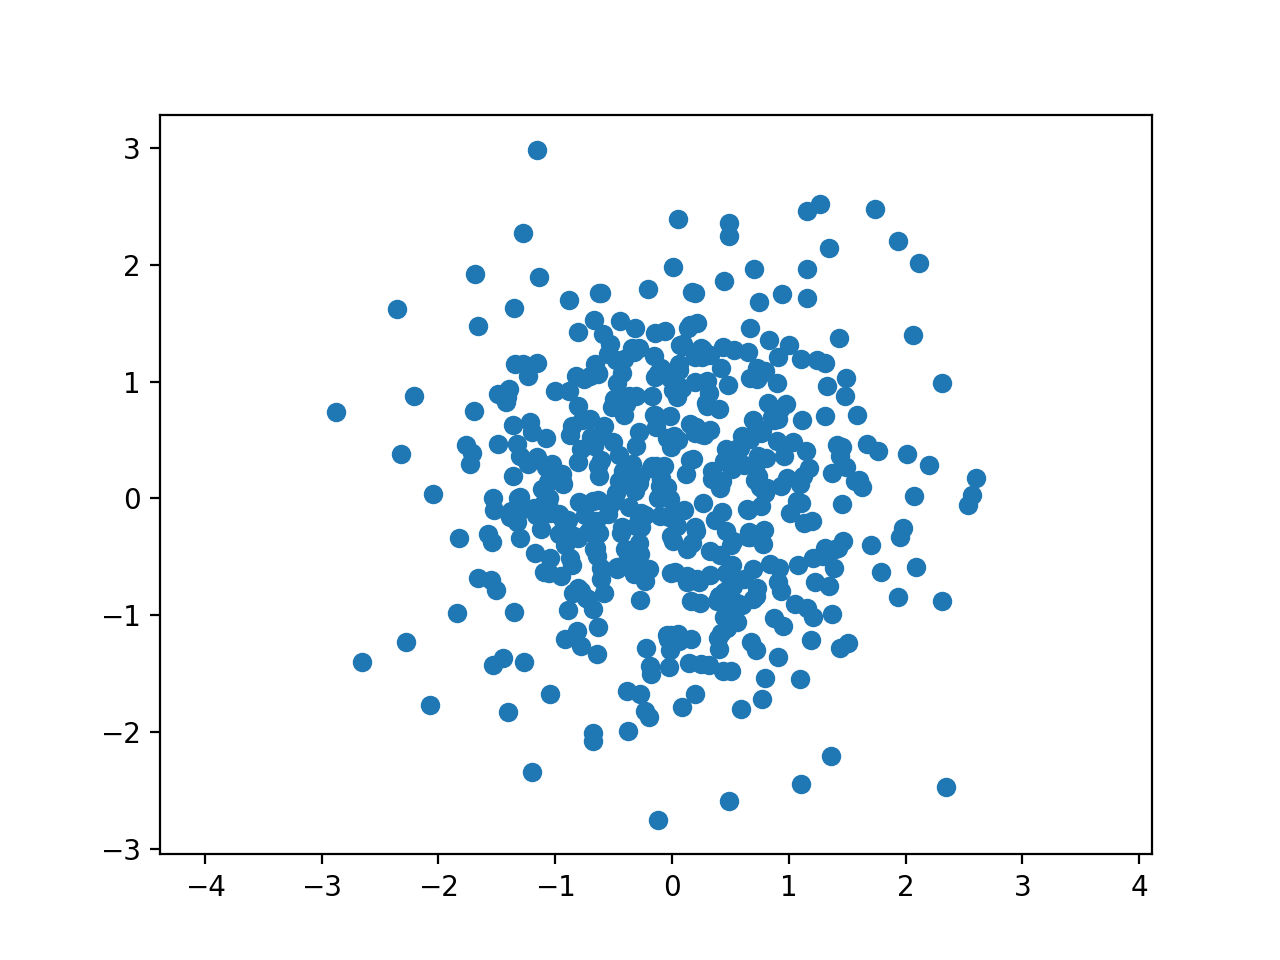
\includegraphics[width=\linewidth]{{fig/e1.1_1}.png}
  \caption*{Uncorrelated}
\endminipage\hfill
\minipage{0.3\textwidth}
    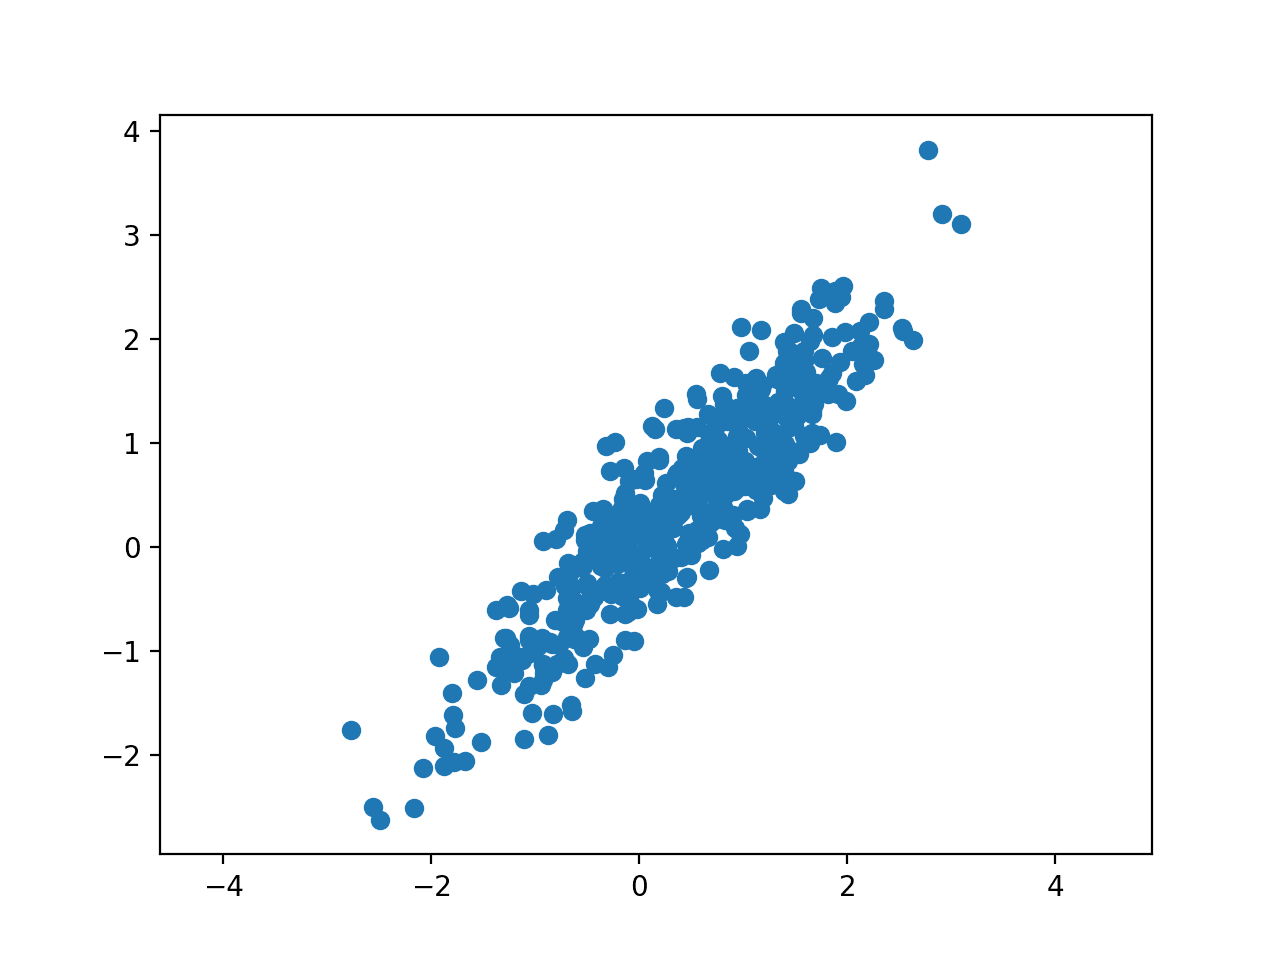
\includegraphics[width=\linewidth]{{fig/e1.1_2}.png}
    \caption*{Correlated}
\endminipage\hfill
\minipage{0.3\textwidth}
    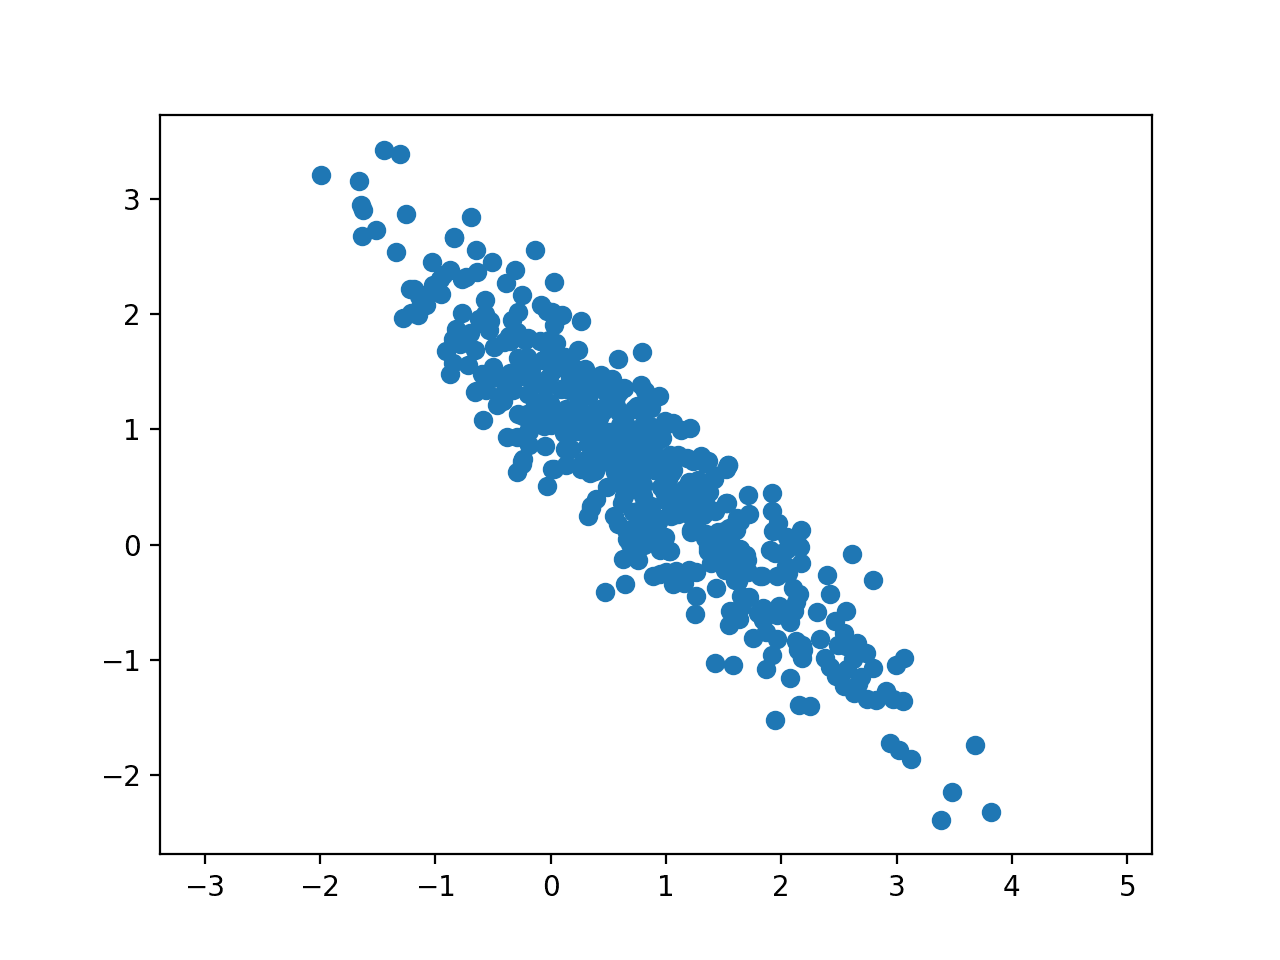
\includegraphics[width=\linewidth]{{fig/e1.1_3}.png}
    \caption*{Anti-correlated}
\endminipage
\end{figure}


\subsection*{1.2.}

Assuming the same $\mu$ and $\Sigma$ setup in \textbf{Exercise 1.1}, we have the $1-, 2-, 3-\sigma$ countour plots being (note eigenvectors are scaled \ilc{4x} for visual purposes):


\begin{figure}[H]
\minipage{0.3\textwidth}
  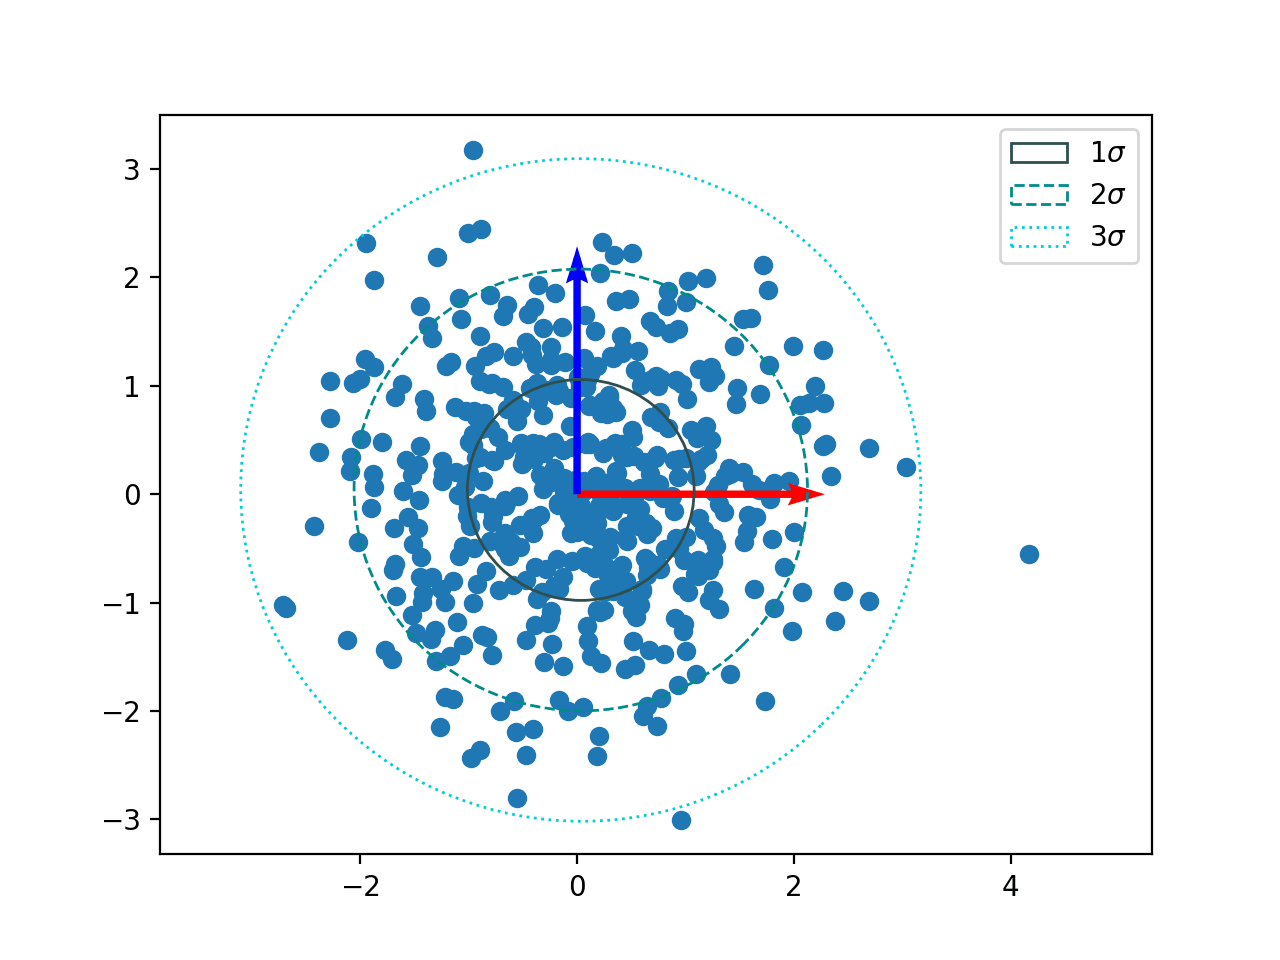
\includegraphics[width=\linewidth]{{fig/e1.2_1}.png}
  \caption*{Uncorrelated}
\endminipage\hfill
\minipage{0.3\textwidth}
    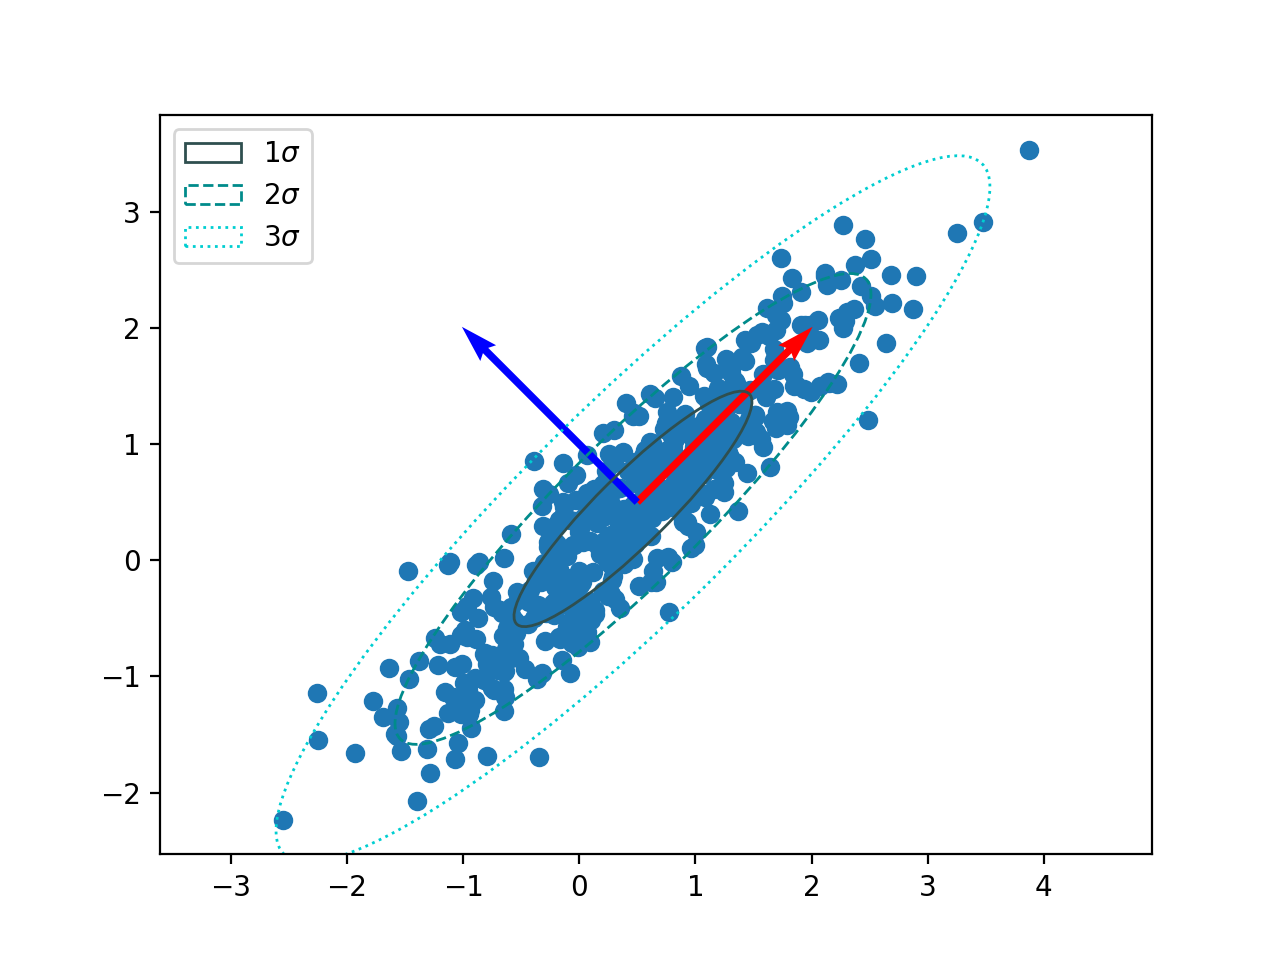
\includegraphics[width=\linewidth]{{fig/e1.2_2}.png}
    \caption*{Correlated}
\endminipage\hfill
\minipage{0.3\textwidth}
    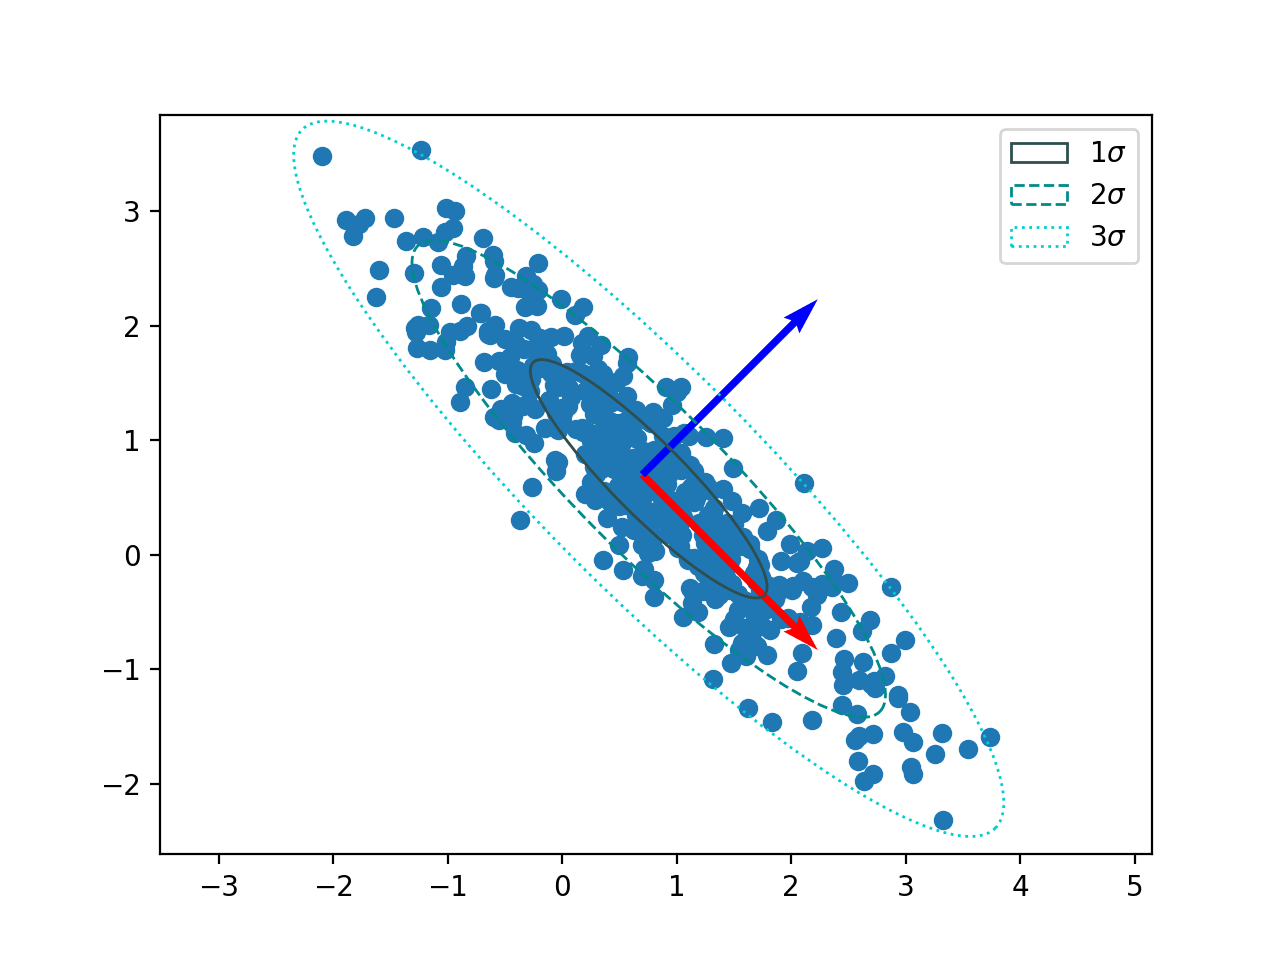
\includegraphics[width=\linewidth]{{fig/e1.2_3}.png}
    \caption*{Anti-correlated}
\endminipage
\end{figure}



\section*{E2. Linear Gaussian Models}

\subsection*{2.1.}
% https://math.stackexchange.com/questions/60911/multivariate-normal-difference-distribution
% https://stats.stackexchange.com/questions/9879/addition-of-multivariate-gaussians

Known the characteristic functions of $x$ and $z$ is:

\begin{align*}
    \phi_x(u) &= \exp(i u^T \mu_x - \frac{1}{2} u^T \Sigma_x u) \\
    \phi_z(u) &= \exp(i u^T \mu_z - \frac{1}{2} u^T \Sigma_z u)
\end{align*}

Since $x$ and $z$ are independent, their sum will still conform to the normal distribution. We may confirm it by analysing the characteristic functions of $x + z$, which is $\phi_{x + z}(u) = E(e^{it(x + z)}) = E(e^{itx}) \cdot E(e^{itz}) = \phi_{x}(u) \phi_{z}(u)$, then we have:

\begin{align*}
    \phi_{x + z}(u) &= \phi_{x}(u) \phi_{z}(u) = \exp(i u^T \mu_x - \frac{1}{2} u^T \Sigma_x u) \cdot \exp(i u^T \mu_z - \frac{1}{2} u^T \Sigma_z u) \\
    &= \exp(i u^T (\mu_x + \mu_z) - \frac{1}{2} u^T (\Sigma_x + \Sigma_z) u) \\
    \Longrightarrow \phi_y(u) &= \exp(i u^T \mu_y - \frac{1}{2} u^T \Sigma_y u)
\end{align*}

Thus, we have $p(y) = \mathcal N(\mu_x+\mu_z,\Sigma_x+\Sigma_z)$.


\subsection*{2.2.}

% https://stats.stackexchange.com/questions/30588/deriving-the-conditional-distributions-of-a-multivariate-normal-distribution
% http://www.math.chalmers.se/~rootzen/highdimensional/SSP4SE-appA.pdf
% http://users.stat.umn.edu/~helwig/notes/norm-Notes.pdf
% https://www.coursera.org/lecture/linear-models-2/normal-conditional-distributions-LiHmE

For clarity, we let $p(x, y) = \mathcal N(\mu, \Sigma)$, where:

\begin{align*}
    \mu &= \qbm{\mu_x \\ \mu_y} \\
    \Sigma &= \qbm{\Sigma_{xx} & \Sigma_{xy} \\ \Sigma_{yx} & \Sigma_{yy}}
\end{align*}

Note each of $\Sigma{ab}$ is a matrix of $a \times b$.

We further know that there must be $p(y \mid x) = \mathcal N(\overline{\mu}, \overline{\Sigma})$, where:

\begin{align*}
    \overline{\mu} &= \mu_y + \Sigma_{yx} \Sigma_{xx}^{-1} (x - \mu_x) \\
    \overline{\Sigma} &= \Sigma_{yy} - \Sigma_{yx} \Sigma_{xx}^{-1}\sigma{yx}
\end{align*}

I don't know if we are expected to show the proof, but here's a trick that can do it rather quickly. Assume $z = y + Ax$ (not to be confused with the $z$ in \textbf{Question 2.1}) with $A = -\Sigma_{yx} \Sigma_{xx}^{-1}$, we have:

\begin{align*}
    cov(z, x) &= cov(y + Ax, x) = cov(y, x) + A \cov(x, x) \\
    &= \Sigma_{yx} + (-\Sigma_{yx} \Sigma_{xx}^-1) \Sigma_{xx} \\
    &\text{Now to deduce $E(y \mid x)$} \\
    \Rightarrow &\begin{cases}
        E(z | x) &= E(z) = E(y + Ax) = \mu_y + A \mu_x = \mu_y -\Sigma_{yx} \Sigma_{xx}^{-1} \mu_x \\
        E(z | x) &= E(y + Ax \mid x) = E(y \mid x) + A E(x \mid x)
    \end{cases} \\
    \Longrightarrow E(y \mid x) &= E(z | x) - A E(x \mid x) = \mu_y -\Sigma_{yx} \Sigma_{xx}^{-1} \mu_x - (-\Sigma_{yx} \Sigma_{xx}^{-1}) x \\
    &= \mu_y + \Sigma_{yx} \Sigma_{xx}^{-1} (x - \mu_x) = \overline{\mu}
\end{align*}


Similarily, we may find out $\overline{\Sigma}$ as (note that $cov(x, y) = cov(y, x)$):


\begin{align*}
    var(y \mid x) &= var(z) = var(y + Ax) \\
    &= var(y) + A var(x) A' + A cov(y, x) + cov(x, y) A' \\
    &= \Sigma_{yy} + \Sigma_{yx} \Sigma_{xx}^{-1} \Sigma_{xx} \Sigma_{xx}^{-1} \Sigma_{xy} - \Sigma_{yx} \Sigma_{xx}^{-1} \Sigma_{yx} - \Sigma_{yx} \Sigma_{xx}^{-1} \Sigma_{xy} \\
    &= \Sigma_{yy} + \Sigma_{yx} \Sigma_{xx}^{-1} \Sigma_{xy} - 2 \Sigma_{yx} \Sigma_{xx}^{-1} \Sigma_{xy} \\
    \Longrightarrow \overline{\Sigma}&= \Sigma_{yy} - \Sigma_{yx} \Sigma_{xx}^{-1} \Sigma_{xy}
\end{align*}


As know from \textbf{Exercise 2.1} that $p(y) = \mathcal N(\mu_x+\mu_z,\Sigma_x+\Sigma_z)$ and $p(x) = \mathcal N(\mu_x, \Sigma_x)$, we have $p(y \mid x) = \mathcal N(\overline{\mu}, \overline{\Sigma})$, where:

\begin{align*}
    \overline{\mu} &= \mu_y + \Sigma_{yx} \Sigma_{xx}^{-1} (x - \mu_x) = \mu_x + \mu_z + \Sigma_{yx} \Sigma_{xx}^{-1} (x - \mu_x) \\
    \overline{\Sigma} &=  \Sigma_{yy} - \Sigma_{yx} \Sigma_{xx}^{-1} \Sigma_{xy} = \Sigma_{x} + \Sigma_{z} -\Sigma_{yx} \Sigma_{xx}^{-1} \Sigma_{xy}
\end{align*}

\subsection*{2.3.}

According to \textbf{Exercise 2.1}, for $y = x + z$, we have $y \sim \mathcal N(\mu_x+\mu_z,\Sigma_x+\Sigma_z)$. For the ease of demo, let $\sigma_x = 3$ and $\sigma_z = 4$ so that we may have the nice $\sigma_x^2 + \sigma_z^2 = \sigma_y^2 \Longleftrightarrow 3^2 + 4^2 = 5^2$ relationship. In such case, we may have:




\begin{align*}
    p(x) &= \mathcal N(\mu_x = 0, \Sigma_x = 3^2) \\
    p(y) &= \mathcal N(\mu_y = 1, \Sigma_y = 4^2) \\
    p(z) &= \mathcal N(\mu_x+\mu_z,\Sigma_x+\Sigma_z) = \mathcal N(\mu_x = 1, \Sigma_x = 5^2)
\end{align*}

The plots will look like:


\begin{figure}[H]
    \centering
    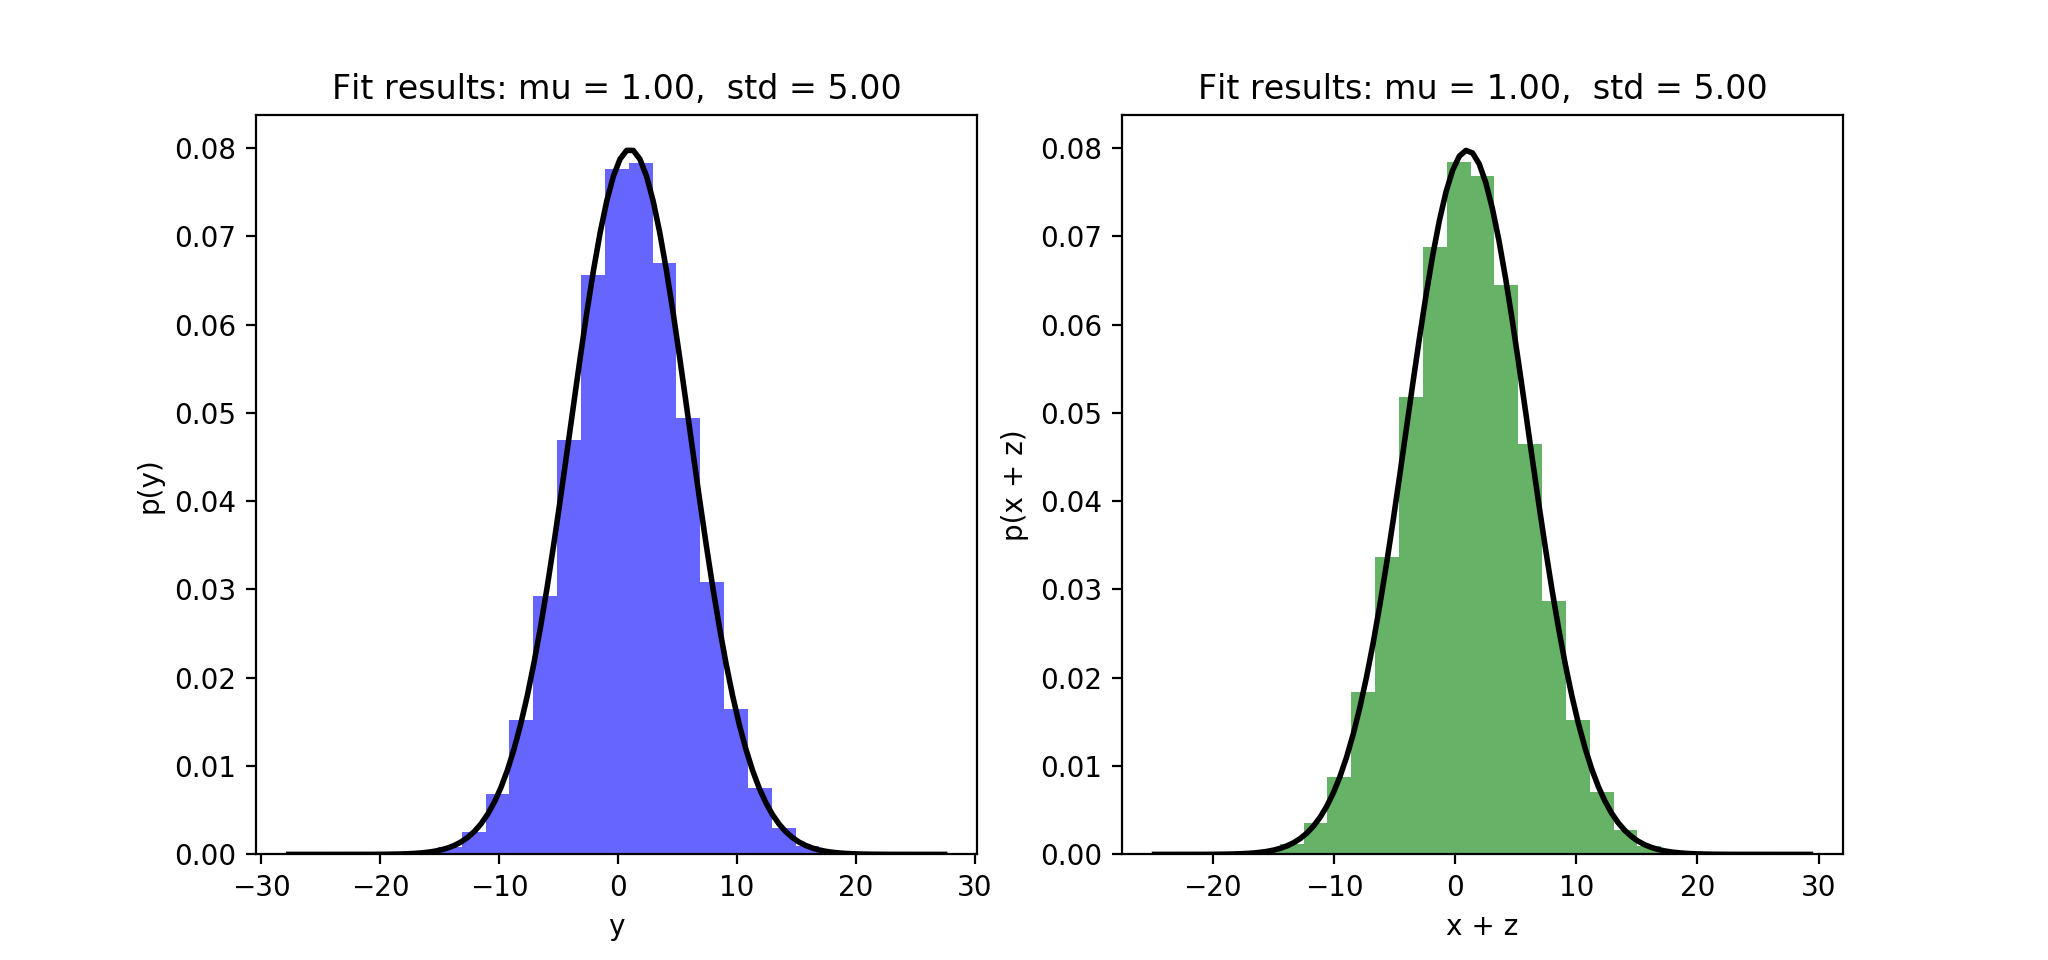
\includegraphics[width=1\linewidth]{{fig/e2.3}.png}
\end{figure}

We may tell these two plots are close resemblance of one and another by inspecting the shape of graph and the parameter of the fitted curve (showed as title of each plot).\newline

Please refer to \ilc{code/p2.py} for the code implementation.

\section*{E3. Dimensionality Reduction and PCA}

\subsection*{3.1.}

The dataset I used in this exercise is the UCI Machine Learning \textit{Glass Classification} dataset I obtained from \href{https://www.kaggle.com/uciml/glass}{Kaggle}.

\begin{lstlisting}
        RI     Na    Mg    Al     Si     K    Ca   Ba   Fe  Type
0  1.52101  13.64  4.49  1.10  71.78  0.06  8.75  0.0  0.0     1
1  1.51761  13.89  3.60  1.36  72.73  0.48  7.83  0.0  0.0     1
2  1.51618  13.53  3.55  1.54  72.99  0.39  7.78  0.0  0.0     1
3  1.51766  13.21  3.69  1.29  72.61  0.57  8.22  0.0  0.0     1
4  1.51742  13.27  3.62  1.24  73.08  0.55  8.07  0.0  0.0     1
...
(214, 10)
\end{lstlisting}

As showned above, it is a dataset of 214 sample, each with 9 attributes, and each sample has a label that belong to 7 of the potential glass types. The attributes is rather straightforward, with \ilc{RI} being refractive index, and all the others are  chemistry elements measured by weight percent in corresponding oxide (e.g. \ilc{Na} is Sodium, \ilc{Mg} is Magnesium, etc). The output labels are something among the lines of \ilc{container}, \ilc{tableware}, and \ilc{headlamps}.

I opted to use this dataset as this is one of the few lightweight datasets with continues variables that I may find, and it has more than 6 dimensions. It probably doesn't make much sense to illustrate the dataset further, but the Kaggle page I linked above has some distribution plots for each element -- if you are interested. One thing to note about this dataset is, due to its lightweight, the dataset is really unbalanced as it has \ilc{70} samples on \ilc{Type 1}, \ilc{76} samples on \ilc{Type 1}, but only \ilc{17, 13, 9, 29} samples on \ilc{Type 3, 5, 6, 7} respectively (yes, \ilc{Type 4: vehicle} is entirely missing).

\subsection*{3.2.}

As we can't nicely plot 9-dimensional data. The first three eigenvalues and their corresponding eigenvectors are:

\begin{lstlisting}
3.00200916e+00 1.65917340e+00 6.79576475e-01

[-9.28126899e-04  1.52290883e-03 -1.37689385e-03  3.10643441e-04
-7.12950233e-04 -1.82174928e-03 -3.32594524e-04 -4.12235755e-03 9.99986948e-01]
[-1.72248332e-02 -3.98797552e-01 -6.54934730e-01 -3.46599960e-01
3.98381798e-01  1.55680962e-02 -3.76900981e-02 -3.62242832e-01 -1.39622177e-03]
[ 7.23534913e-01  5.43050989e-01 -1.31198879e-01 -9.86931157e-02
-7.68490459e-02  4.77602532e-02 -7.49534298e-02 -3.75274748e-01 -1.84522571e-03]
\end{lstlisting}

First we may confirm that the eigenvalues are indeed sorted in decreasing order, suggesting an eigenvalue with smaller index implies greater squared sum of variances and therefore accounts for higher percentage of variation.

We may also confirm that these eigenvectors are indeed 9-dimensional as expected, and they are orthognal to eachother as the inner products between them yield 0:

\begin{lstlisting}
<v_1, v_2> = 4.336808689942018e-19
<v_2, v_3> = -5.551115123125783e-17
<v_1, v_3> = -4.336808689942018e-19
\end{lstlisting}
(There are not exactly zero due to datatype accuracy problem, but with at least $10^{-17}$ they are close enough to zero.)

\subsection*{3.3.}

\begin{figure}[H]
    \centering
    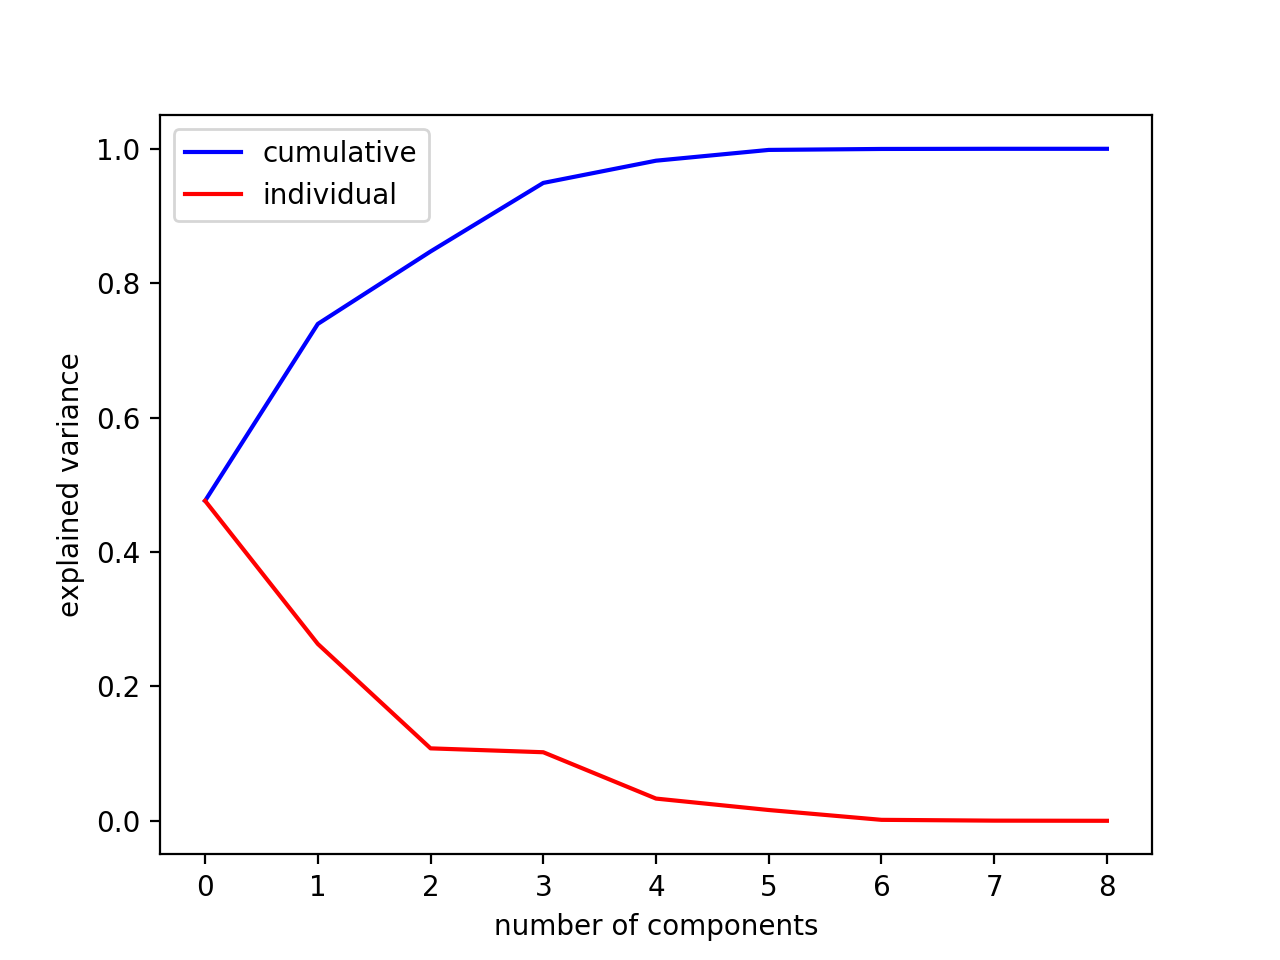
\includegraphics[width=0.5\linewidth]{{fig/e3.3}.png}
\end{figure}

The \textcolor{red}{red} line represents the percentage of variation that particular principle component accounts for. In this case, as we are ploting with respect to the decreasing order of eigenvalues, each principle component accountss for less variation than the previous one. Reversely, the \textcolor{blue}{blue}, whic represents the cumulative variance, is increasing as we add in more principle components -- and when we have all principle components (which is the dimension of the attributes or number of samples, in this case it is the former) considered, the cummulative explained variance reaches 1.

\subsection*{3.4.}

By reducing the dataset to 2 dimensions (\ilc{PC1, PC2}) -- meaning that these two eigenvectors has the two largest eigenvalues, suggesting the range of data projection are more distinguishiable on these two eigenvectors and therefore they contain most information -- we may have the following plot. Note the data were standardized with respect to their mean in this plot and throughout the PCA process, so that we won't have one catagory of data dominating all the others:

\begin{figure}[H]
    \centering
    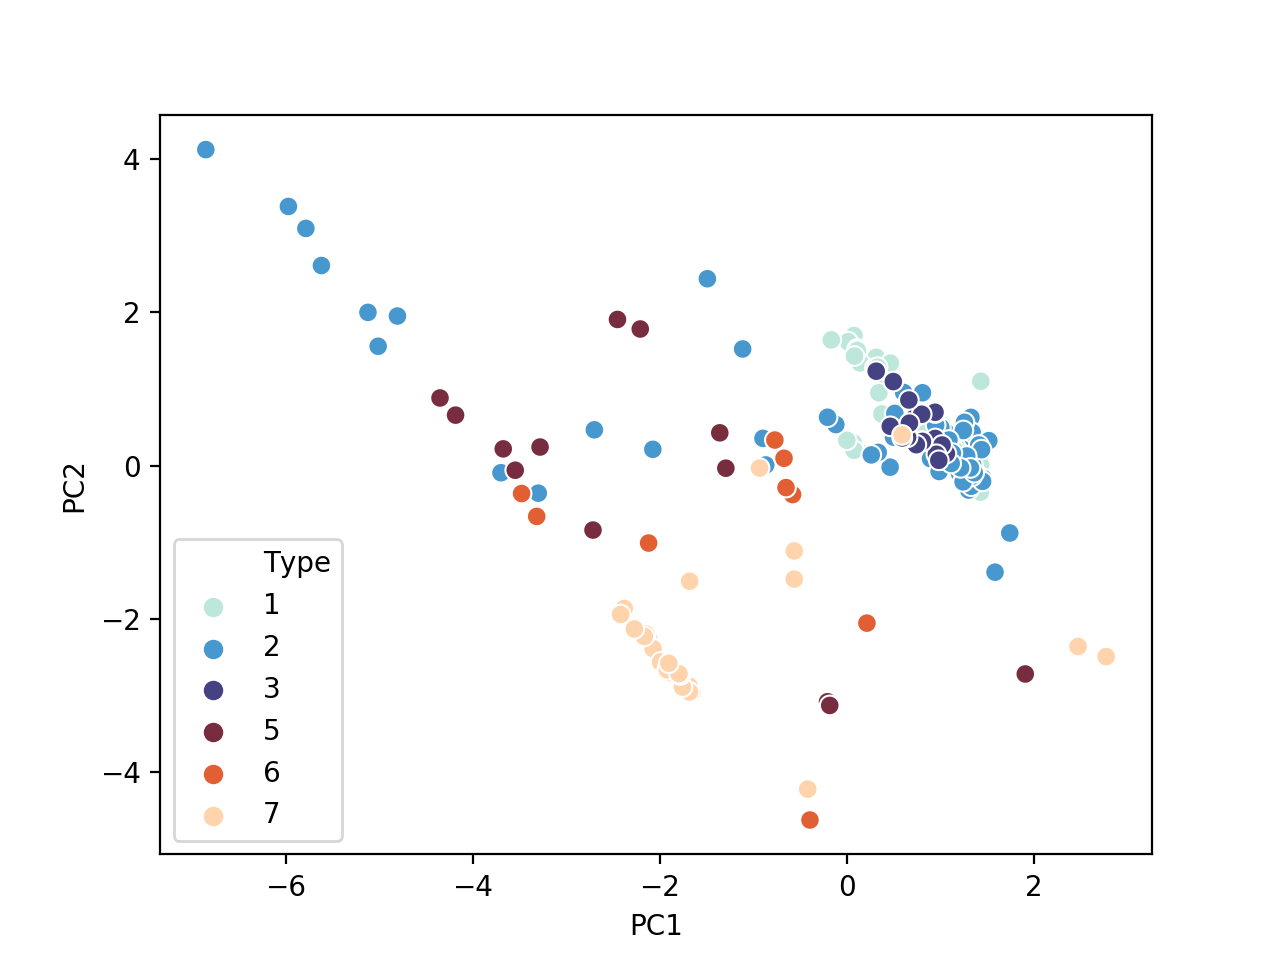
\includegraphics[width=0.7\linewidth]{{fig/e3.4_1}.png}
\end{figure}

I guess we may say the first two principle components perform pretty well on \ilc{Type 7} glass, but not much the others, especially between \ilc{Type 1, 2, 3}, a zoom in plot will look like this:

\begin{figure}[H]
    \centering
    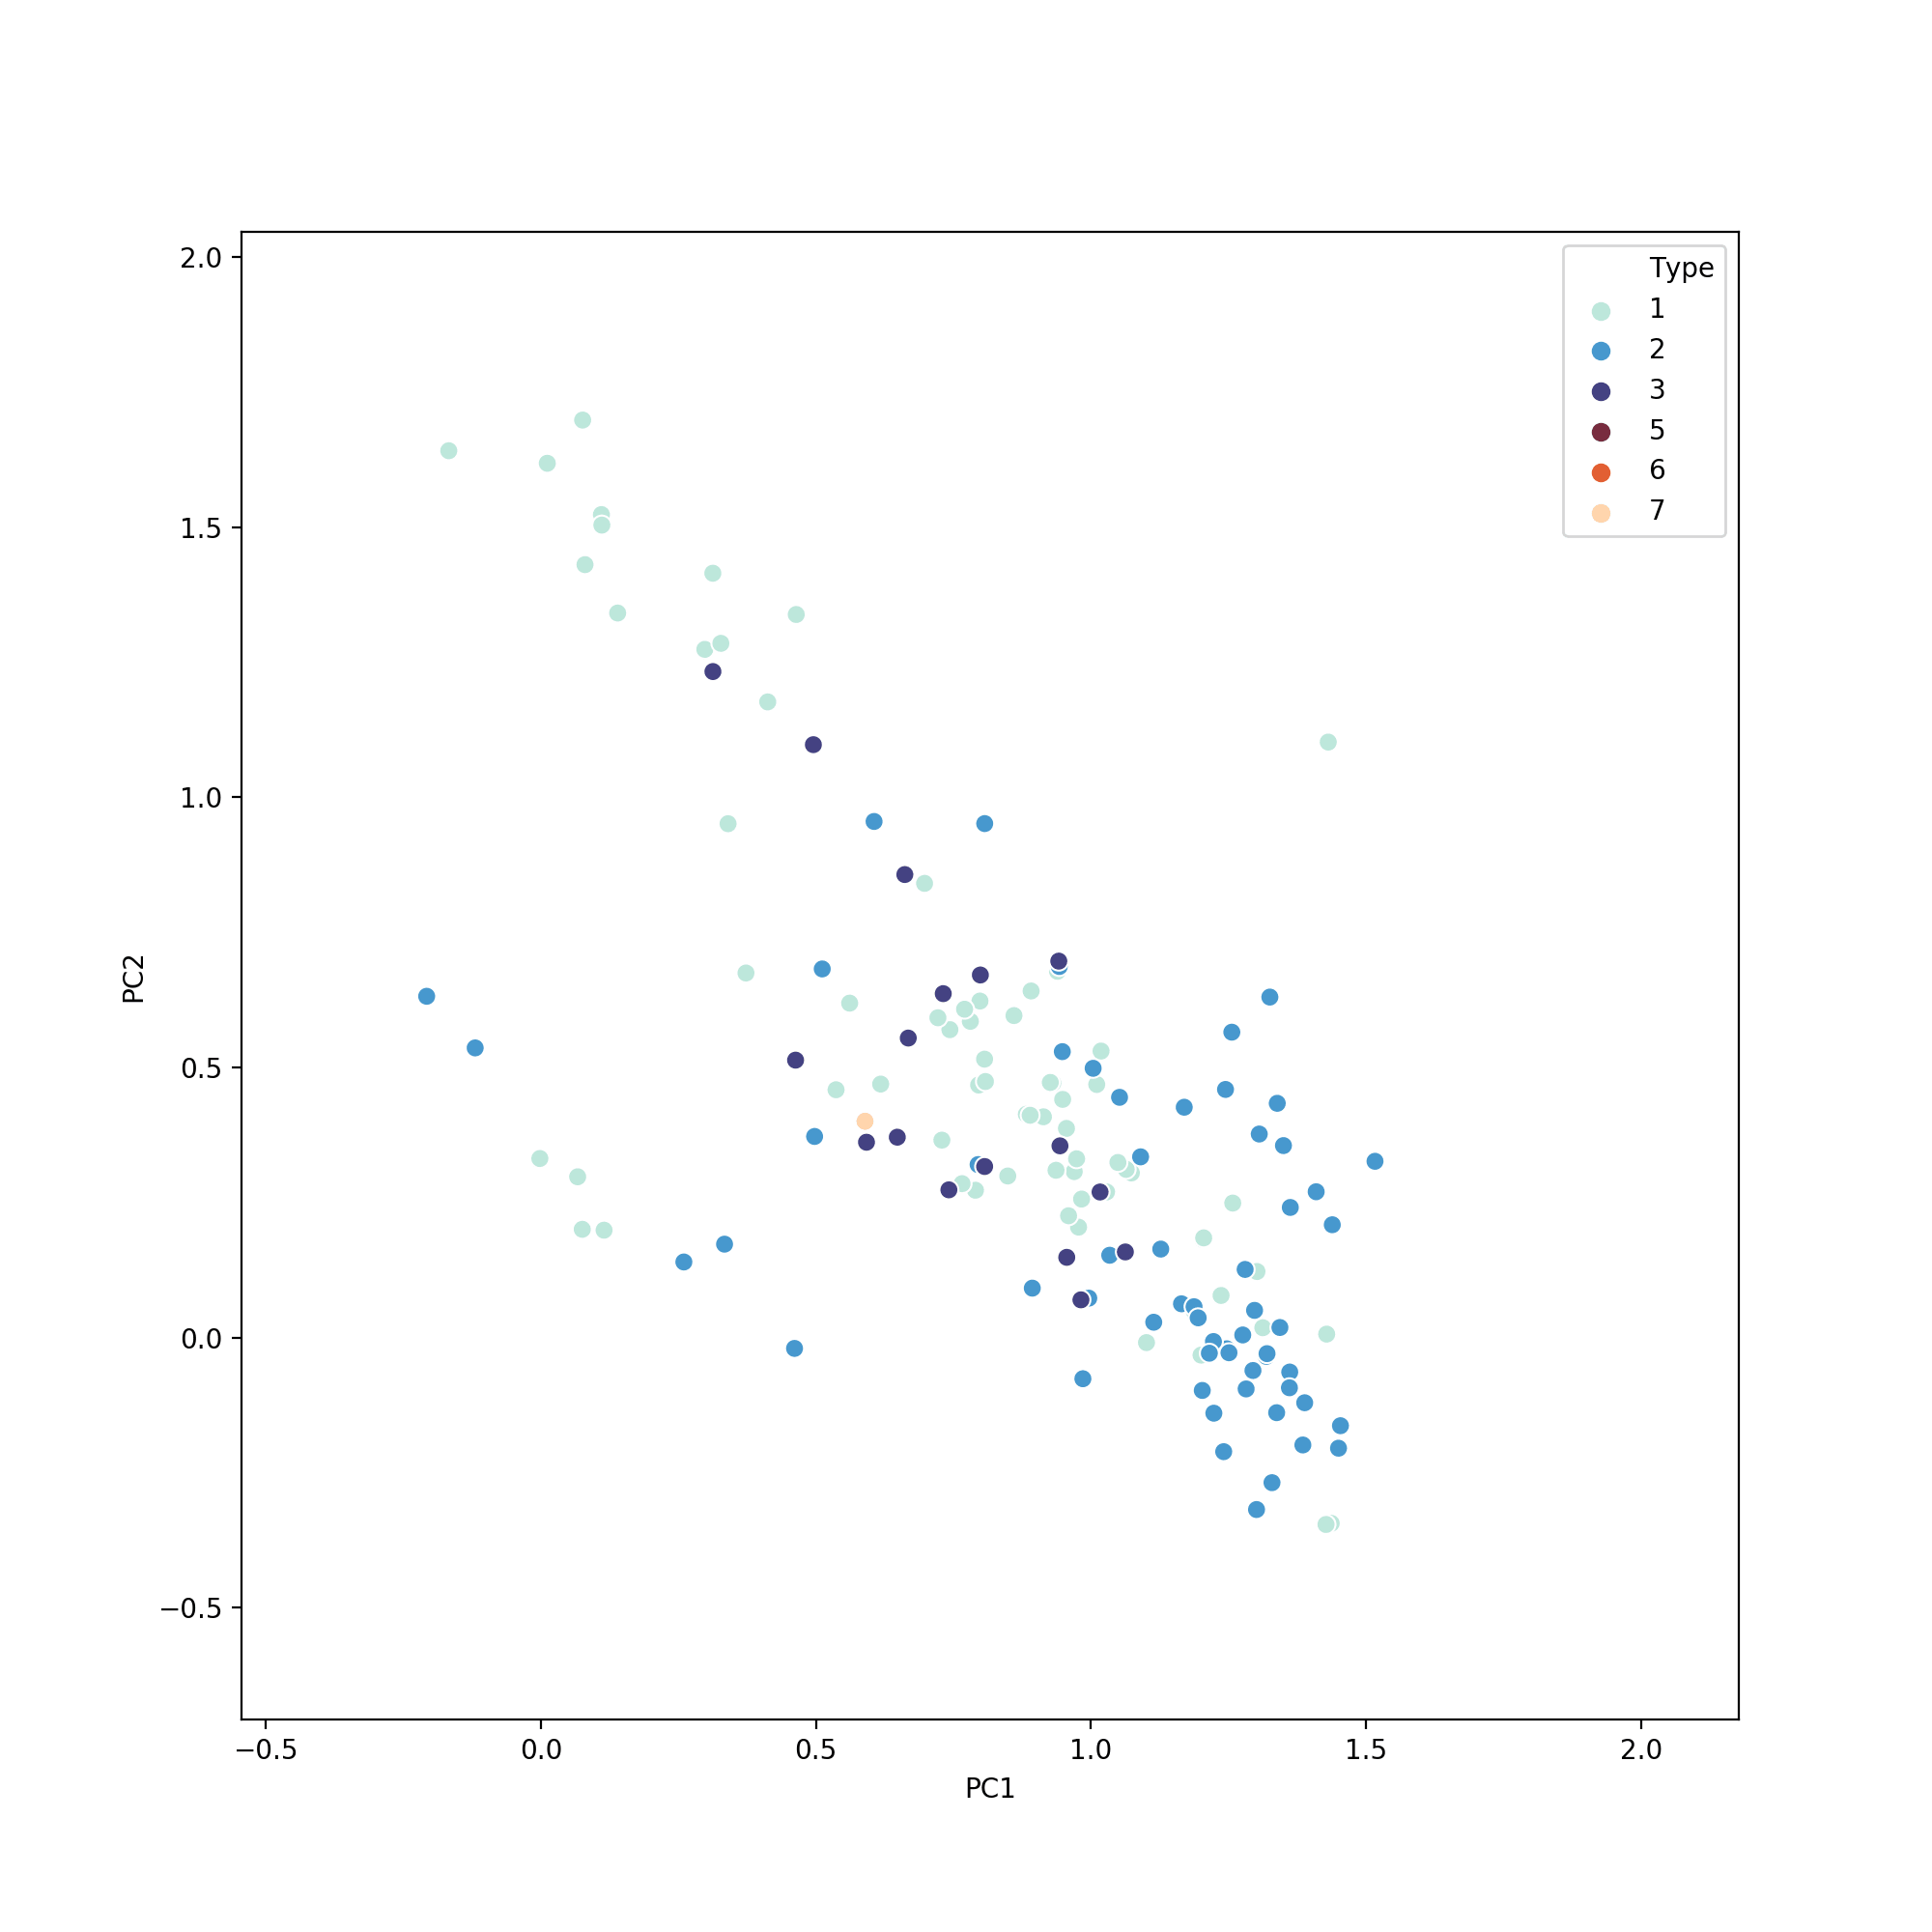
\includegraphics[width=0.5\linewidth]{{fig/e3.4_2}.png}
\end{figure}

This is something rather expected as we have 7 output labels (in fact, 6 output labels as we have no \ilc{Type 4}), but only 2 dimensions to project the clustering. The performance is further limited due to the unbalanced nature of having significantly more \ilc{Type 1} and \ilc{Type 2} samples, granting \ilc{Type 1\&2} glasses to display more features that are potentially similar to other types of glasses (just like doing multiple testing).




\section*{E4. Gaussian Mixture Models }

\section*{Exploration}

% https://www.youtube.com/watch?v=NEaUSP4YerM
% https://medium.com/@violante.andre/an-introduction-to-t-sne-with-python-example-47e6ae7dc58f


\end{document}

